\documentclass[xcolor=pdftex,dvipsnames,table]{UT}

\usepackage{amsthm}
\usepackage{tikz}
\usepackage{eurosym}
\usepackage{graphicx}
\usepackage{kbordermatrix}
\usepackage{subcaption}


\newcommand{\pinspins}{pins2pins}
\newcommand{\mcrl}{mCRL2}
\newcommand{\promela}{Promela}
\newcommand{\prob}{prob}
\newcommand{\dve}{DVE}
\newcommand{\uppaal}{Uppaal}
\newcommand{\ltsmin}{LTSmin}
\newcommand{\pins}{PINS}
\newcommand{\animo}{ANIMO}

\usetikzlibrary{arrows, automata}
\newtheorem{mydef}{Definition}

\background{1}	% choose background {1..5}
\taal{EN} 	%EN or NL

\title{Symbolic Model Checking of Timed Automata using LTSmin}
\subtitle{Sybe van Hijum}
\date{\today} 

\begin{document} 

\maketitleslide

%Choose a sideway banner, choose (side1, side2, side3, side4, side5)
\setbeamertemplate{background}{\includegraphics[width=0.1\paperwidth,height=\paperheight]{img/side5}} 

%includes the acutal text of the files.
  % DO NOT COMPILE THIS FILE DIRECTLY!
% This is included by the other .tex files.

\section{Introduction}

\begin{frame}{Model Checking}
\begin{itemize}
	
	\item {\large  Models a system, program, protocol, etc...}
	\item {\large  Check if model meets specifications}
	\item {\large  Problem: State space explosion}
	\begin{itemize}
		\item {\large Grows exponentially with size of model}
	\end{itemize}
	\item {\large Timed Automata adds time to these models}
\end{itemize}
\end{frame}

\begin{frame}{Research Problems}
Problem: Model checkers are designed for discrete variables (integers), clocks have real values.
\begin{itemize}
\item Can we use the LTSmin symbolic model checker for timed automata?
\item Can we optimize the symbolic back end for clocks?
\end{itemize}
\end{frame}


\begin{comment}
\begin{frame}{Transition System}
\begin{figure}
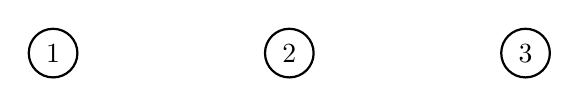
\begin{tikzpicture}[->,>=stealth',shorten >=1pt,auto,node distance=3cm,
                    thick,main node/.style={circle,draw}]

  \node[main node] (1) {1};
  \node[main node] (2) [right of=1] {2};
  \node[main node] (3) [right of=2] {3};
  
\end{tikzpicture}
\end{figure}
\end{frame}

\begin{frame}{Transition System}
\begin{figure}
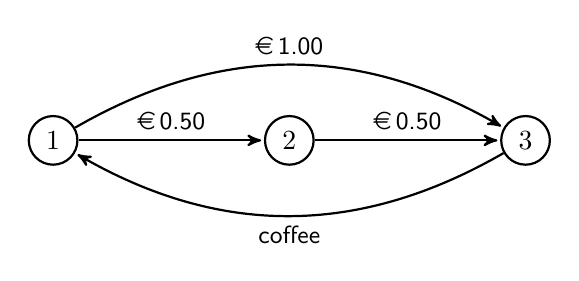
\begin{tikzpicture}[->,>=stealth',shorten >=1pt,auto,node distance=3cm,
                    thick,main node/.style={circle,draw}]

  \node[main node] (1) {1};
  \node[main node] (2) [right of=1] {2};
  \node[main node] (3) [right of=2] {3};

  \path[every node/.style={font=\sffamily\small}]
    (1) edge node [above] {\EUR{0.50}} (2)
        edge [bend left] node[above] {\EUR{1.00}} (3)
    (2) edge node [above] {\EUR{0.50}} (3)
    (3) edge [bend left] node [below] {coffee} (1);

\end{tikzpicture}
\end{figure}
\end{frame}

\begin{frame}{Transition System}
\begin{figure}
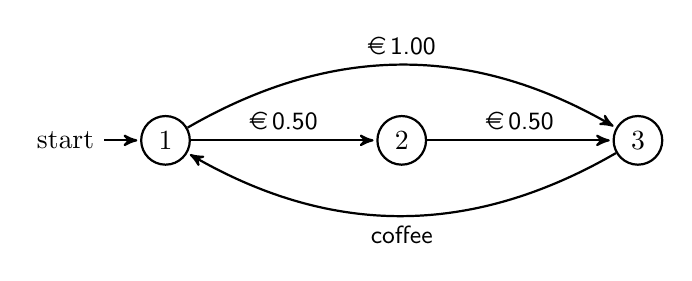
\begin{tikzpicture}[->,>=stealth',shorten >=1pt,auto,node distance=3cm,
                    thick,main node/.style={circle,draw}]

  \node[initial, main node] (1) {1};
  \node[main node] (2) [right of=1] {2};
  \node[main node] (3) [right of=2] {3};

  \path[every node/.style={font=\sffamily\small}]
    (1) edge node [above] {\EUR{0.50}} (2)
        edge [bend left] node[above] {\EUR{1.00}} (3)
    (2) edge node [above] {\EUR{0.50}} (3)
    (3) edge [bend left] node [below] {coffee} (1);
\end{tikzpicture}
\end{figure}
\end{frame}
\end{comment}

\begin{comment}
\begin{frame}{Transition System}
\begin{mydef}[Labeled Transition System]
A labeled transition system is a 3-tuple A = $\langle S, Act, s_o \rangle$ where
\begin{itemize}
\item $S$ is a finite set of states
\item $Act$ is a finite set of labelled actions
\item $s_o \in S$ is a finite set of actions
\end{itemize}
\end{mydef}
\end{frame}


\begin{frame}{Timed Automata}
\begin{mydef}[Timed Automata]
\label{def:TA}
An extended timed automaton is a 6-tuple A = $\langle L, C, Act, l_0, \rightarrow, I_c\rangle$ where
	\begin{itemize}
		\item L is a finite set of locations, typically denoted by $l$
		\item C is a finite set of clocks, typically denoted by c
		\item Act is a finite set of actions
		\item $l_0 \in$ L is the initial location
		\item $\rightarrow \subseteq L \times G(C) \times Act \times 2^C \times L$ is the (non-deterministic) transition relation.
		\item $I_C : L \rightarrow G(C)$ is a function mapping locations to downwards closed clock invariants.
	\end{itemize}
\end{mydef}
\end{frame}
\end{comment}

\begin{frame}{Transition System}

\includegraphics[height=0.85\textheight, width=.95\textwidth, keepaspectratio=true]{img/Koffie_states}
\end{frame}

\begin{frame}{Transition System}
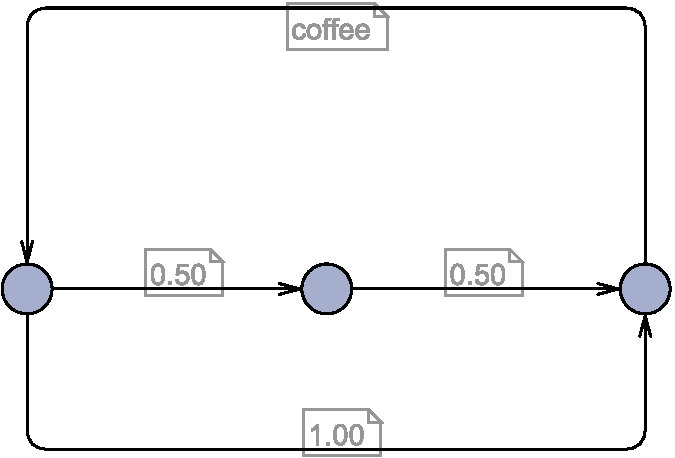
\includegraphics[height=0.85\textheight, width=.95\textwidth, keepaspectratio=true]{img/Koffie_states_transitions}
\end{frame}

\begin{frame}{Transition System}
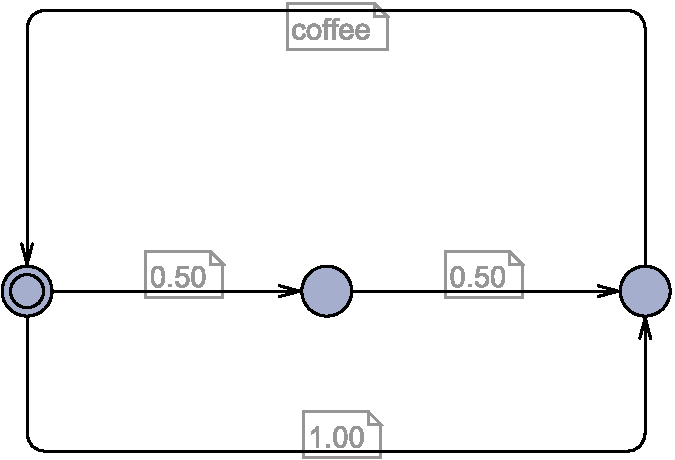
\includegraphics[height=0.85\textheight, width=.95\textwidth, keepaspectratio=true]{img/Koffie_automaton}
\end{frame}

\begin{frame}{Timed Automata}
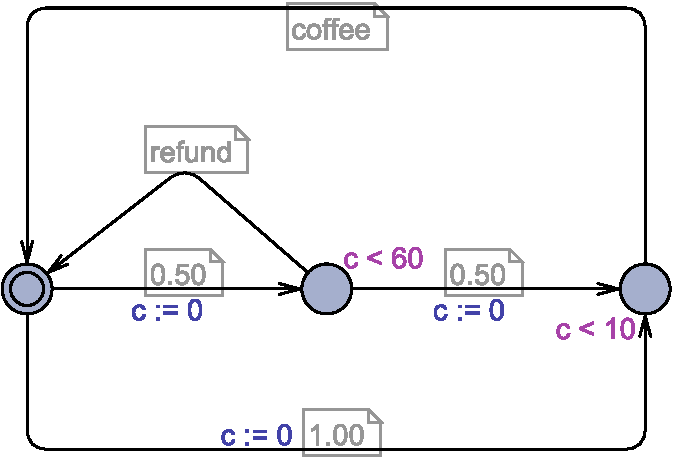
\includegraphics[height=0.85\textheight, width=.95\textwidth, keepaspectratio=true]{img/Koffie_complete}
\end{frame}



\begin{comment}
\begin{frame}{Boolean Decision Diagram}
	\begin{itemize} 
		\item Expresses boolean expressions 
		\item States can be seen as boolean expressions 
		\item Memory efficient
	\end{itemize} 
\end{frame}

\begin{frame}{Boolean Decision Diagram}
\begin{figure}[h]
\centering
	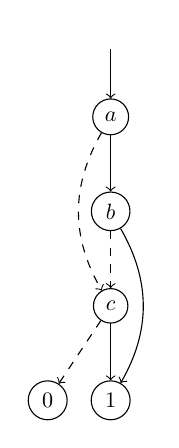
\begin{tikzpicture}[
		smallvertex/.style={circle,draw,scale=0.8}
		]
		\node[smallvertex](S1){$a$};
		\node[smallvertex, draw = none, above of = S1, yshift = 0.25cm](S0){};
		
		\node[smallvertex, below of = S1, yshift = -.5cm](S2){$b$};
		\node[smallvertex, below of = S2, yshift = -.5cm](S3){$c$};
		\node[smallvertex, below of = S3, yshift = -.5cm](S4){$1$};
		\node[smallvertex, left of = S4](S5){$0$};
		
		\draw[->] (S0) --(S1) node [midway, above, sloped, scale=0.75,
		rotate=0, xshift =-0.4 cm, yshift = -0.2cm]{};
		\draw[->] (S1) --(S2) node [midway, above, sloped, scale=0.75,
		rotate=90, xshift =-0.4 cm, yshift = -0.2cm]{};
		\draw[dashed,->] (S2) --(S3) node [midway, above, sloped, scale=0.75,
		rotate=90, xshift =-0.4 cm, yshift = -0.2cm]{};
		\draw[->] (S3) --(S4) node [midway, above, sloped, scale=0.75,
		rotate=90, xshift =-0.4 cm, yshift = -0.2cm]{};		
		\draw[->,dashed] (S1) edge[bend right](S3) node [midway, above, sloped, scale=0.75,
		rotate=90, xshift =-0.4 cm, yshift = -0.2cm]{};	
		\draw[->] (S2) edge[bend left](S4) node [midway, above, sloped, scale=0.75,
		rotate=90, xshift =-0.4 cm, yshift = -0.2cm]{};	
		\draw[dashed,->] (S3) --(S5) node [midway, above, sloped, scale=0.75,
		rotate=90, xshift =-0.4 cm, yshift = -0.2cm]{};
		[bend left]
	\end{tikzpicture}
\caption{A BDD representing $(a \wedge b) \vee c$}
\label{fig:BDD}
\end{figure}
\end{frame}


\begin{frame}{LTSmin}
	\begin{itemize} 
		\item Language independent model checker
		\item Multiple algorithmic back ends
		\item Internal optimization wrappers	
	\end{itemize} 
\end{frame}	
	
\begin{frame}{LTSmin}
\begin{figure}[width=\textwidth] 
\scalebox{0.65}{\input{img/pins}}
\end{figure}
\end{frame}

\end{comment}



\section{Time Zones}


\begin{frame}{Time Zones}
Time not represented as a variable, but as a zone. Most used structure to represent zones: Different Bound Matrix (DBM)
\begin{itemize}
	\item Only convex zones
	\item Memory inefficient
\end{itemize}
\begin{center}
\includegraphics[width=0.25\textwidth]{img/TA}
\end{center}
\begin{figure}
\centering
	\begin{subfigure}{0.3\textwidth}
	\centering
		$0 \leq c < 60$
		
		$\Downarrow$		
		
		$c - 0 < 60$
		
		$0 - c \leq 0 $
	\end{subfigure}
	\begin{subfigure}{0.3\textwidth}
	\begin{math}
 \bordermatrix{ 	   & \mathbf{O}    & c         \cr
 			\mathbf{O} &(0,\leq)       & (0,\leq)  \cr
 			c          &(60,<   )      & (0,\leq)  \cr}
	\end{math}
	\end{subfigure}
\end{figure}
\end{frame}

\begin{frame}
\begin{figure}
	\centering
	\begin{math}
% 		\begin{pmatrix}
 \bordermatrix{ 		                 & \mathbf{O} & c_1           & c_2        \cr
 			\mathbf{O} &(0,\leq)      & (0,\leq)      & (0,\leq)     \cr
 			c_1        &(5,<)      & (0,\leq)      & (5,<)\cr
 			c_2        &(5,<)      & (5,<) & (0,\leq)     \cr}
% 		\end{pmatrix}
	\end{math}
\end{figure}

\begin{figure}[h]
\centering
\scalebox{0.65}{
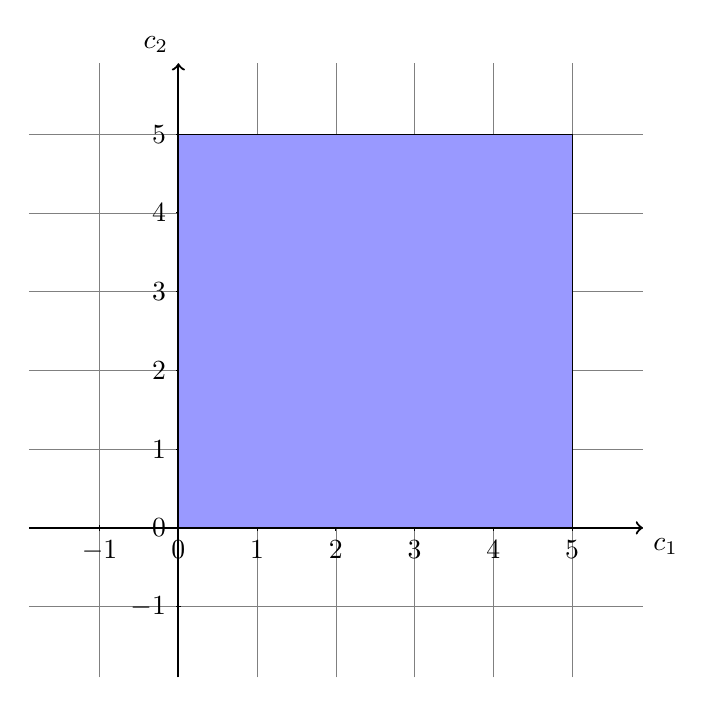
\begin{tikzpicture}

\draw[step=1cm,gray,very thin] (-1.9,-1.9) grid (5.9,5.9);

%\shadedraw[inner color=blue,outer color=red, draw=black] (0,0) rectangle (4,4);

\draw[thick,->] (-1.9,0) -- (5.9,0) node[anchor=north west] {$c_1$};
\draw[thick,->] (0,-1.9) -- (0,5.9) node[anchor=south east] {$c_2$};

\foreach \x in {-1,0,1,2,3,4,5}
    \draw (\x cm,1pt) -- (\x cm,-1pt) node[anchor=north] {$\x$};
\foreach \y in {-1,0,1,2,3,4,5}
    \draw (1pt,\y cm) -- (-1pt,\y cm) node[anchor=east] {$\y$};
    
\filldraw[fill=blue!40!white, draw=black] (0,0) rectangle (5,5);
\end{tikzpicture}
}
\end{figure}
\end{frame}


\section{LDD solution}

\begin{comment}
\begin{frame}{Current LTSmin Uppaal setup}
\includegraphics[width=\textwidth]{img/opaal}
\end{frame}
\end{comment}



\begin{comment}
\begin{frame}{List Decision Diagram}

\begin{mydef}[List Decision Diagram]
A List Decision Diagram (LDD) is a directed acyclic graph $(V,E)$. The vertex set $V$ contains two terminals $0$ and $1$ with out-degree zero, and a set of non-terminal vertices with out-degree two and the following attributes.
%\\\\
\begin{tabular}{lll}
Attribute                & Type                      & Description                                           \\\hline
var(v)                   & \textbf{Var}              & Variable x \\

const(v)                 & $\mathbb{Z}$              & Constant c.                                           \\
high(v), low(v)          & $V$                       & High-branch h, and low-branch l.                   
\end{tabular}
\captionof*{table}{}  
The set E contains the edges $(v,low(v))$ and $(v, high(v))$, where $v \in V$ is a non-terminal vertex.
\end{mydef} 

\end{frame}
\end{comment}

\begin{frame}{List Decision Diagram}
\begin{figure}
\begin{subfigure}[b]{.4\textwidth}
	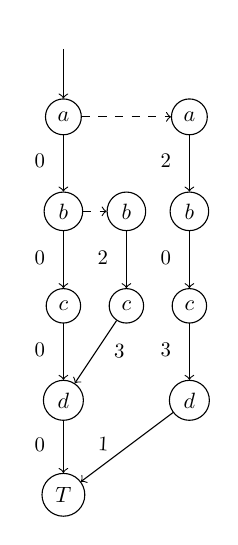
\begin{tikzpicture}[
		smallvertex/.style={circle,draw,scale=0.8}
		]
		\node[smallvertex](S1){$a$};
		\node[smallvertex, draw = none, above of = S1, yshift = 0.25cm](S0){};
		
		\node[smallvertex, below of = S1, yshift = -.5cm](S2){$b$};
		\node[smallvertex, below of = S2, yshift = -.5cm](S3){$c$};
		\node[smallvertex, below of = S3, yshift = -.5cm](S4){$d$};
		\node[smallvertex, below of = S4, yshift = -.5cm](S5){$T$};
		\node[smallvertex, right of = S2](S6){$b$};
		\node[smallvertex, right of = S3](S7){$c$};
		\node[smallvertex, right of = S6](S9){$b$};
		\node[smallvertex, above of = S9, yshift = .5cm](S8){$a$};
		\node[smallvertex, below of = S9, yshift = -.5cm](S10){$c$};
		\node[smallvertex, below of = S10, yshift = -.5cm](S11){$d$};
		
		\draw[->] (S0) --(S1) node [midway, above, sloped, scale=0.75,
		rotate=0, xshift =-0.4 cm, yshift = -0.2cm]{};
		\draw[->] (S1) --(S2) node [midway, above, sloped, scale=0.75,
		rotate=90, xshift =-0.4 cm, yshift = -0.2cm]{$0$};
		\draw[->] (S2) --(S3) node [midway, above, sloped, scale=0.75,
		rotate=90, xshift =-0.4 cm, yshift = -0.2cm]{$0$};
		\draw[->] (S3) --(S4) node [midway, above, sloped, scale=0.75,
		rotate=90, xshift =-0.4 cm, yshift = -0.2cm]{$0$};
		\draw[->] (S4) --(S5) node [midway, above, sloped, scale=0.75,
		rotate=90, xshift =-0.4 cm, yshift = -0.2cm]{$0$};
		\draw[dashed, ->] (S2) --(S6) node [midway, above, sloped, scale=0.75,
		rotate=90, xshift =-0.4 cm, yshift = -0.2cm]{};
		\draw[->] (S6) --(S7) node [midway, above, sloped, scale=0.75,
		rotate=90, xshift =-0.4 cm, yshift = -0.2cm]{$2$};
		\draw[->] (S7) --(S4) node [midway, above, sloped, scale=0.75,
		rotate=300, xshift =0.4 cm, yshift = -0.2cm]{$3$};
		\draw[dashed, ->] (S1) --(S8) node [midway, above, sloped, scale=0.75,
		rotate=90, xshift =-0.4 cm, yshift = -0.2cm]{};
		\draw[->] (S8) --(S9) node [midway, above, sloped, scale=0.75,
		rotate=90, xshift =-0.4 cm, yshift = -0.2cm]{$2$};
		\draw[->] (S9) --(S10) node [midway, above, sloped, scale=0.75,
		rotate=90, xshift =-0.4 cm, yshift = -0.2cm]{$0$};
        \draw[->] (S10) --(S11) node [midway, above, sloped, scale=0.75,
		rotate=90, xshift =-0.4 cm, yshift = -0.2cm]{$3$};
		\draw[->] (S11) --(S5) node [midway, above, sloped, scale=0.75,
		rotate=320, xshift =-0.4 cm, yshift = -0.2cm]{$1$};


	\end{tikzpicture}
	\end{subfigure}
	\begin{subfigure}[b]{.4\textwidth}
		\begin{itemize}
			\item Diagram to represent set of valuations of integer variables
			\item Each node has high and low edge
			\item Each level represents a variable
			\item Order of variables important
		\end{itemize}
	\end{subfigure}
\label{fig:ldd-example}
\end{figure}
\end{frame}

\begin{frame}{Breadth First Search}

\begin{algorithmic}[1]
\Procedure{BFS}{$initial$}
	\State $vis := cur := initial$
	\While{$cur \neq \emptyset$}
		\State{$cur := next(cur)$}
		\State{$cur := cur \setminus vis$}
		\State{$vis := vis \cup cur$}
	\EndWhile
	
\EndProcedure	
\end{algorithmic}

\end{frame}

\begin{frame}{DBM into state vector}
\begin{figure}
	\centering
	\begin{math}
% 		\begin{pmatrix}
 \bordermatrix{ 		                 & \mathbf{O} & c_1           & c_2        \cr
 			\mathbf{O} &(0,\leq)      & (0,\leq)      & (0,\leq)     \cr
 			c_1        &(5,<)      & (0,\leq)      & (5,<)\cr
 			c_2        &(5,<)      & (5,<) & (0,\leq)     \cr}
% 		\end{pmatrix}
	\end{math}
\end{figure}


\begin{itemize}
	\item Old situation
	\begin{itemize}
		\item $\{l_0,...,l_n,ptr\}$
	\end{itemize}
	\item New situation
	\begin{itemize}
		\item $\{l_0,...,l_n,(0,\leq),(0,\leq),(5,<),(5,<),(5,<),(5,<)\}$
	\end{itemize}
\end{itemize}
\end{frame}

\begin{comment}
\begin{frame}{LTSmin}
	\begin{itemize}
		\item States as integer vectors
	 	\item Partitioned next-state function
	 	\item Optimizations based on matrices
	 	\begin{itemize}
	 		\item Read(r)
	 		\item Must-write(w)
	 		\item May-write(W)
	 		\item Copy(-)
	 	\end{itemize}
	\end{itemize}
\end{frame}


\begin{frame}{Matrices}
\begin{center}
    \begin{tabular}{lll}
    1: & $x = 1 \vee a[1] = 0$ & $\rightarrow a[1] := 1, x:=0 , y:=5$  \\
    2: & $a[0] = 1 \vee y = 5$                     & $\rightarrow a[x] := 0, x:= 1$ \\
    \end{tabular}
\end{center}

\begin{figure}[h]
\centering
	\begin{math}
 \kbordermatrix{ 		               & x & y & a[0] & a[1] \cr
 									  1& + & w & -    & +    \cr
 									  2& + & r & +    & W    \cr}
	\end{math}
%	\caption{Dependency Matrix}
%	\label{fig:dep_matrix}
\end{figure}
\end{frame}

\end{comment}

\begin{frame}{LDD solution}
\begin{itemize}
	\item Correct, working solution
	\item Variable reordering possible
	\item All variables seen as discrete values
	\item No optimizations based on time
\end{itemize}
\end{frame}

\section{DDD Solution}

\begin{comment}
\begin{frame}{Difference Decision Diagram}
\begin{mydef}[Difference Decision Diagram]
A difference decision diagram (DDD) is a directed acyclic graph $(V,E)$. The vertex set $V$ contains two terminals $0$ and $1$ with out-degree zero, and a set of non-terminal vertices with out-degree two and the following attributes.
\\
\scalebox{0.85}{
\begin{tabular}{lll}
Attribute                & Type                      & Description                                           \\\hline
pos(v), neg(v)           & \textbf{Var}              & Positive variable $x_i$, and negative variable $x_j$. \\
op(v)                    & $\{<$, $\leq\}$     & Operator $<$ or $\leq$.                         \\
const(v)                 & $\mathbb{D}$              & Constant c.                                           \\
high(v), low(v)          & $V$                       & High-branch h, and low-branch l.                   
\end{tabular}}
The set E contains the edges $(v,low(v))$ and $(v, high(v))$, where $v \in V$ is a non-terminal vertex.
\end{mydef}
\end{frame}
\end{comment}

\begin{frame}
\begin{figure}
\begin{subfigure}{0.45\textwidth}
\begin{subfigure}{\textwidth}
\scalebox{0.50}{
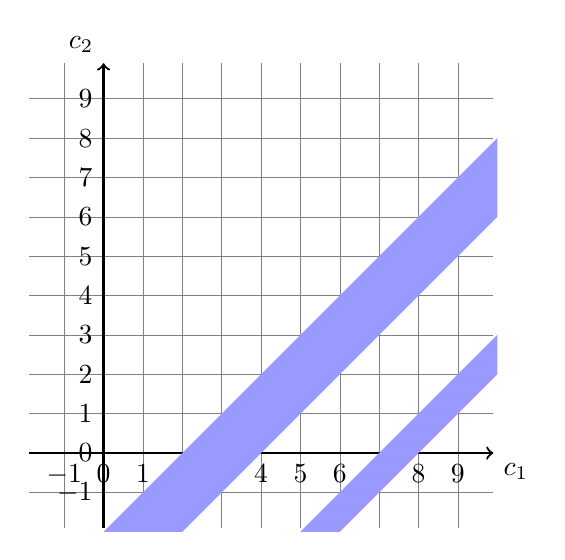
\begin{tikzpicture}[scale=0.5]

\draw[step=1cm,gray,very thin] (-1.9,-1.9) grid (9.9,9.9);
\draw[thick,->] (-1.9,0) -- (9.9,0) node[anchor=north west] {$c_1$};
\draw[thick,->] (0,-1.9) -- (0,9.9) node[anchor=south east] {$c_2$};

\foreach \x in {-1,0,1,2,3,4,5,6,7,8,9}
    \draw (\x cm,1pt) -- (\x cm,-1pt) node[anchor=north] {$\x$};
\foreach \y in {-1,0,1,2,3,4,5,6,7,8,9}
    \draw (1pt,\y cm) -- (-1pt,\y cm) node[anchor=east] {$\y$};

\fill[fill=blue!40!white] (5,-2) -- (10,3) -- (10,2) -- (6,-2) -- (5,-2);

\fill[fill=blue!40!white] (0,-2) -- (2,-2) -- (10,6) -- (10,8) -- (0,-2);
    
%\filldraw[fill=blue!40!white, draw=black] (0,0) rectangle (5,5);
\end{tikzpicture}}
\end{subfigure}

\begin{subfigure}{\textwidth}
	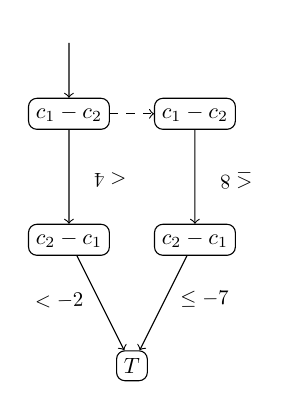
\begin{tikzpicture}[
		smallvertex/.style={rectangle,rounded corners=3pt,draw,scale=0.8}
		]
			
		\node[smallvertex](S0){$c_1 - c_2$};
		\node[smallvertex, draw = none, above of = S0, yshift = 0.25cm](S5){};
		\draw[->] (S5) --(S0) node [midway, above, sloped, scale=0.75,
		rotate=295, xshift =-0.4 cm, yshift = -0.2cm]{};
		\node[smallvertex, right of = S0, xshift = 1cm](S1){$c_1 - c_2$};
		\draw[dashed,->] (S0) --(S1) node [midway, above, sloped, scale=0.75,
		rotate=0, xshift =-0.7 cm, yshift = -0.2cm]{};
		\node[smallvertex, below of = S0, yshift = -1cm](S2){$c_2 - c_1$};
		\draw[->] (S0) --(S2) node [midway, above, sloped, scale=0.75,
		rotate=90, xshift =-0.7 cm, yshift = -0.2cm]{$< 4$};
		\node[smallvertex, below of = S1, yshift = -1cm](S3){$c_2 - c_1$};
		\draw[->] (S1) --(S3) node [midway, above, sloped, scale=0.75,
		rotate=90, xshift =-0.7 cm, yshift = -0.2cm]{$\leq 8$};
		\node[smallvertex, below of = S0, xshift = 1cm, yshift = -3cm](S4){$T$};
		\draw[->] (S2) --(S4) node [midway, above, sloped, scale=0.75,
		rotate=65, xshift =-0.7 cm, yshift = -0.2cm]{$<-2$};
		\draw[->] (S3) --(S4) node [midway, above, sloped, scale=0.75,
		rotate=297, xshift =0.7 cm, yshift = -0.2cm]{$\leq-7$};
	\end{tikzpicture}
	\end{subfigure}
\end{subfigure}
\begin{subfigure}{0.5\textwidth}
Difference Decision Diagram
\begin{itemize}
	\item Structure like LDD
	\item Added difference operator to each node
	\item Operator $<$ or $\leq$
\end{itemize}
\end{subfigure}
\end{figure}
\end{frame}

\begin{frame}{Ordering}
\begin{mydef}[Ordered DDD]
An ordered DDD (ODDD) is a DDD where each non-terminal vertex $v$ satisfies:
\begin{enumerate}
  \item $neg(v) \prec pos(v)$,
  \item $var(v) \prec var(high(v))$,
  \item $var(v) \prec var(low(v))$ or \\ $var(v) = var(low(v))$ and $bound(v) \prec bound(low(v))$.
\end{enumerate}
\end{mydef}

\begin{figure}[h]
	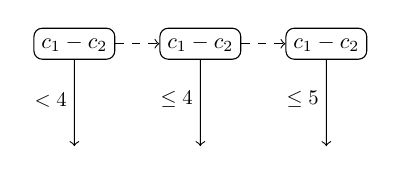
\begin{tikzpicture}[
		smallvertex/.style={rectangle,rounded corners=3pt,draw,scale=0.8}
		]
			
		\node[smallvertex](S0){$c_1 - c_2$};
		\node[smallvertex, right of = S0, xshift = 1cm](S1){$c_1 - c_2$};
		\node[smallvertex, right of = S1, xshift = 1cm](S2){$c_1 - c_2$};
		\node[smallvertex, draw = none, below of = S0, yshift = -0.75cm](S3){};
		\node[smallvertex, draw = none, below of = S1, yshift = -0.75cm](S4){};
		\node[smallvertex, draw = none, below of = S2, yshift = -0.75cm](S5){};
		\draw[->] (S0) --(S3) node [midway, above, sloped, scale=0.75,
		rotate=270, xshift =-0.4 cm, yshift = -0.2cm]{$< 4$};
		\draw[->] (S1) --(S4) node [midway, above, sloped, scale=0.75,
		rotate=270, xshift =-0.4 cm, yshift = -0.2cm]{$\leq 4$};
		\draw[->] (S2) --(S5) node [midway, above, sloped, scale=0.75,
		rotate=270, xshift =-0.4 cm, yshift = -0.2cm]{$\leq 5$};
		\draw[dashed,->] (S0) --(S1) node [midway, above, sloped, scale=0.75,
		rotate=0, xshift =-0.7 cm, yshift = -0.2cm]{};
		\draw[dashed,->] (S1) --(S2) node [midway, above, sloped, scale=0.75,
		rotate=0, xshift =-0.7 cm, yshift = -0.2cm]{};

	\end{tikzpicture}
\end{figure}

\end{frame}


\begin{frame}
\begin{mydef}[Locally Reduced DDD]
A locally reduced DDD ($R_LDDD$) is an ODDD satisfying, for all non-terminals u and v:
\begin{enumerate}
  \item $\mathbb{D} = \mathbb{Z}$ implies $\forall v. op(v) = '\leq'$,
  \item $(cstr(u),high(u),low(u)) = (cstr(v),high(v),low(v))$ implies $u = v$,
  \item $low(v) \neq high(v)$,
  \item $var(v) = var(low(v))$ implies $high(v) \neq high(low(v))$.
\end{enumerate}
\end{mydef}

\begin{figure}[h]
\begin{center}
	\scalebox{0.9}{
	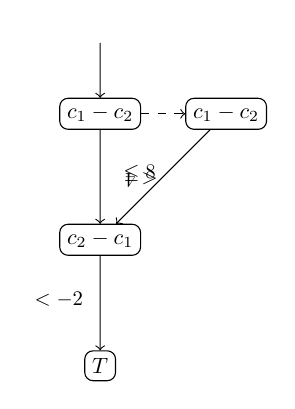
\begin{tikzpicture}[
		smallvertex/.style={rectangle,rounded corners=3pt,draw,scale=0.8}
		]
			
		\node[smallvertex](S0){$c_1 - c_2$};
		\node[smallvertex, draw = none, above of = S0, yshift = 0.25cm](S5){};
		\draw[->] (S5) --(S0) node [midway, above, sloped, scale=0.75,
		rotate=295, xshift =-0.4 cm, yshift = -0.2cm]{};
		\node[smallvertex, right of = S0, xshift = 1cm](S1){$c_1 - c_2$};
		\draw[dashed,->] (S0) --(S1) node [midway, above, sloped, scale=0.75,
		rotate=0, xshift =-0.7 cm, yshift = -0.2cm]{};
		\node[smallvertex, below of = S0, yshift = -1cm](S2){$c_2 - c_1$};
		\draw[->] (S0) --(S2) node [midway, above, sloped, scale=0.75,
		rotate=90, xshift =-0.7 cm, yshift = -0.2cm]{$< 4$};
		\draw[->] (S1) --(S2) node [midway, above, sloped, scale=0.75,
		rotate=315, xshift =-0.4 cm, yshift = -0.2cm]{$\leq 8$};
		\node[smallvertex, below of = S0, yshift = -3cm](S4){$T$};
		\draw[->] (S2) --(S4) node [midway, above, sloped, scale=0.75,
		rotate=270, xshift =-0.7 cm, yshift = -0.2cm]{$<-2$};
	\end{tikzpicture}
	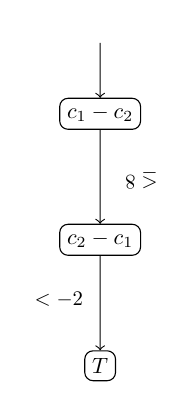
\begin{tikzpicture}[
		smallvertex/.style={rectangle,rounded corners=3pt,draw,scale=0.8}
		]
			
		\node[smallvertex](S0){$c_1 - c_2$};
		\node[smallvertex, draw = none, above of = S0, yshift = 0.25cm](S5){};
		\draw[->] (S5) --(S0) node [midway, above, sloped, scale=0.75,
		rotate=295, xshift =-0.4 cm, yshift = -0.2cm]{};
		\node[smallvertex, below of = S0, yshift = -1cm](S2){$c_2 - c_1$};
		\draw[->] (S0) --(S2) node [midway, above, sloped, scale=0.75,
		rotate=90, xshift =-0.7 cm, yshift = -0.2cm]{$\leq 8$};
		\node[smallvertex, below of = S0, yshift = -3cm](S4){$T$};
		\draw[->] (S2) --(S4) node [midway, above, sloped, scale=0.75,
		rotate=270, xshift =-0.7 cm, yshift = -0.2cm]{$<-2$};
	\end{tikzpicture}}
\end{center}
\end{figure}

\end{frame}

\begin{frame}{DDD Nodes}
A node contains two 40 bit pointers, 32 bit value, type, operator and flag bit

Node is stored as a 128 bit struct, two 64 bit integers

Total information is 115 bit, 13 unused bits, all set to 0

%\begin{lstlisting} 
%struct dddnode {
%    uint64_t a, b;
%} * dddnode_t; 
%\end{lstlisting}

\begin{figure}
\centering
\begin{bytefield}[bitwidth=1.2em]{16}
  \bitbox{5}{low edge}
  \bitbox{1}{\rule{\width}{\height}}
  \bitbox{4}{value}
  \bitbox{1}{\rule{\width}{\height}}
  \bitbox{5}{high edge}\\
\end{bytefield}
\end{figure}

\end{frame}

\begin{frame}{Minus}
\begin{figure}[ht]

\begin{subfigure}[h]{.3\textwidth}
\scalebox{0.3}{
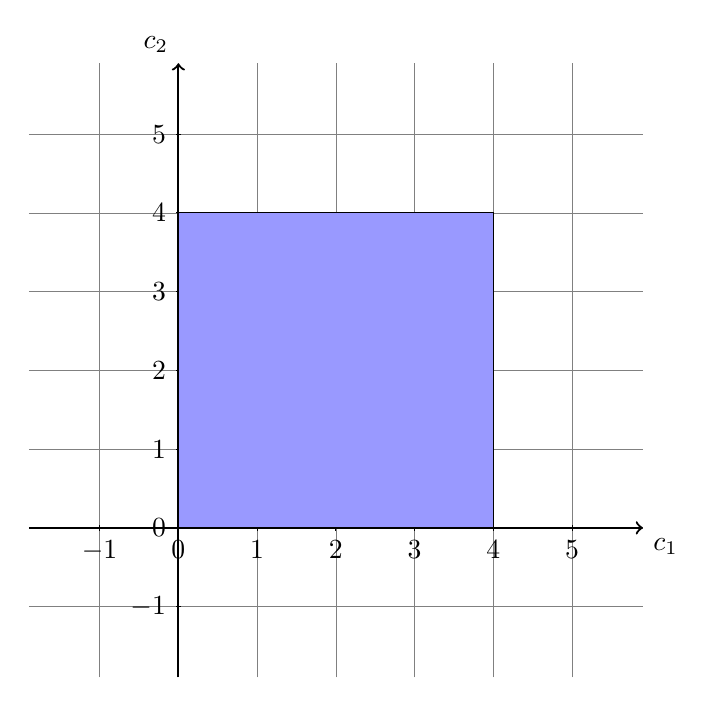
\begin{tikzpicture}

\draw[step=1cm,gray,very thin] (-1.9,-1.9) grid (5.9,5.9);

%\shadedraw[inner color=blue,outer color=red, draw=black] (0,0) rectangle (4,4);

\draw[thick,->] (-1.9,0) -- (5.9,0) node[anchor=north west] {$c_1$};
\draw[thick,->] (0,-1.9) -- (0,5.9) node[anchor=south east] {$c_2$};

\foreach \x in {-1,0,1,2,3,4,5}
    \draw (\x cm,1pt) -- (\x cm,-1pt) node[anchor=north] {$\x$};
\foreach \y in {-1,0,1,2,3,4,5}
    \draw (1pt,\y cm) -- (-1pt,\y cm) node[anchor=east] {$\y$};
    
\filldraw[fill=blue!40!white, draw=black] (0,0) rectangle (4,4);

\end{tikzpicture}}
\end{subfigure}
\begin{subfigure}[h]{.3\textwidth}
\scalebox{0.3}{
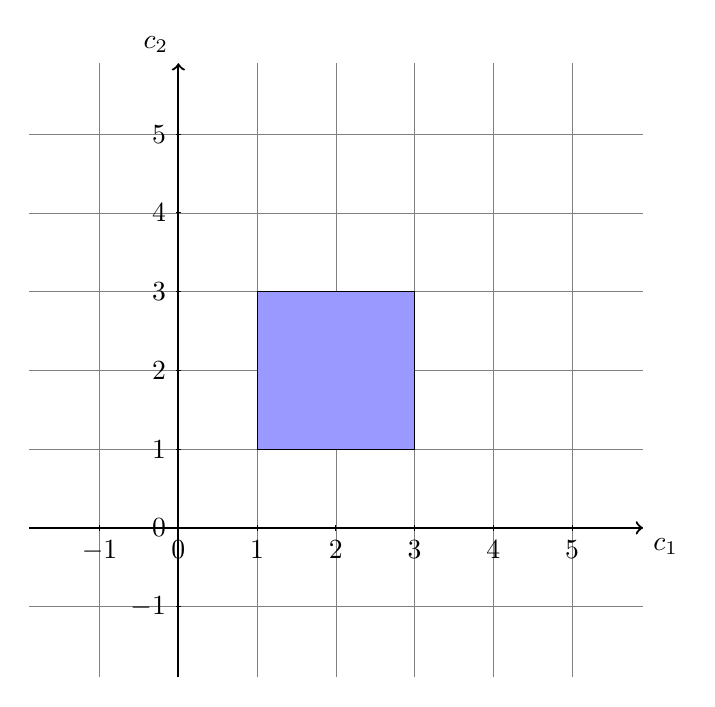
\begin{tikzpicture}
\draw[step=1cm,gray,very thin] (-1.9,-1.9) grid (5.9,5.9);

%\shadedraw[inner color=blue,outer color=red, draw=black] (0,0) rectangle (4,4);

\draw[thick,->] (-1.9,0) -- (5.9,0) node[anchor=north west] {$c_1$};
\draw[thick,->] (0,-1.9) -- (0,5.9) node[anchor=south east] {$c_2$};

\foreach \x in {-1,0,1,2,3,4,5}
    \draw (\x cm,1pt) -- (\x cm,-1pt) node[anchor=north] {$\x$};
\foreach \y in {-1,0,1,2,3,4,5}
    \draw (1pt,\y cm) -- (-1pt,\y cm) node[anchor=east] {$\y$};
    
\filldraw[fill=blue!40!white, draw=black] (1,1) rectangle (3,3);

\end{tikzpicture}}
\end{subfigure}
\begin{subfigure}[h]{.3\textwidth}
\scalebox{0.3}{
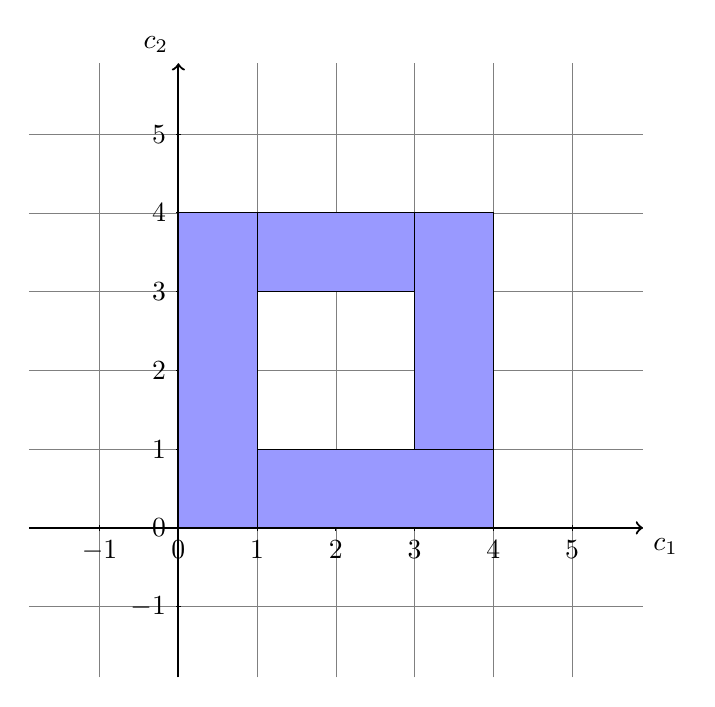
\begin{tikzpicture}
\draw[step=1cm,gray,very thin] (-1.9,-1.9) grid (5.9,5.9);

%\shadedraw[inner color=blue,outer color=red, draw=black] (0,0) rectangle (4,4);

\draw[thick,->] (-1.9,0) -- (5.9,0) node[anchor=north west] {$c_1$};
\draw[thick,->] (0,-1.9) -- (0,5.9) node[anchor=south east] {$c_2$};

\foreach \x in {-1,0,1,2,3,4,5}
    \draw (\x cm,1pt) -- (\x cm,-1pt) node[anchor=north] {$\x$};
\foreach \y in {-1,0,1,2,3,4,5}
    \draw (1pt,\y cm) -- (-1pt,\y cm) node[anchor=east] {$\y$};
    
\filldraw[fill=blue!40!white, draw=black] (0,3) rectangle (4,4);
\filldraw[fill=blue!40!white, draw=black] (3,0) rectangle (4,4);
\filldraw[fill=blue!40!white, draw=black] (0,0) rectangle (4,1);
\filldraw[fill=blue!40!white, draw=black] (0,0) rectangle (1,4);

\end{tikzpicture}}
\end{subfigure}

\end{figure}

Difference of two convex zones not always convex
\end{frame}

\begin{frame}{Minus}
\begin{figure}
	\begin{subfigure}{0.2\textwidth}
	\scalebox{0.8}{
	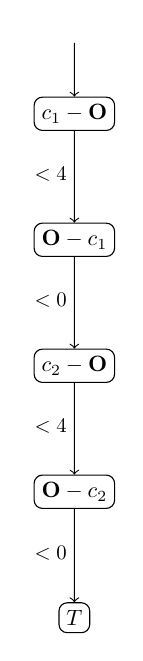
\begin{tikzpicture}[
		smallvertex/.style={rectangle,rounded corners=3pt,draw,scale=0.8}
		]		
		\node[smallvertex](S1){$c_1 - \mathbf{O}$};
		\node[smallvertex, draw = none, above of = S1, yshift = 0.25cm](S0){};
		\node[smallvertex, below of = S1, yshift = -1cm](S2){$\mathbf{O} - c_1$};
		\node[smallvertex, below of = S2, yshift = -1cm](S3){$c_2 - \mathbf{O}$};
		\node[smallvertex, below of = S3, yshift = -1cm](S4){$\mathbf{O} - c_2$};
		\node[smallvertex, below of = S4, yshift = -1cm](S5){$T$};
		
		\draw[->] (S0) --(S1) node [midway, above, sloped, scale=0.75,
		rotate=0, xshift =-0.4 cm, yshift = -0.2cm]{};
		\draw[->] (S1) --(S2) node [midway, above, sloped, scale=0.75,
		rotate=270, xshift =-0.4 cm, yshift = -0.2cm]{$<4$};
		\draw[->] (S2) --(S3) node [midway, above, sloped, scale=0.75,
		rotate=270, xshift =-0.4 cm, yshift = -0.2cm]{$<0$};
		\draw[->] (S3) --(S4) node [midway, above, sloped, scale=0.75,
		rotate=270, xshift =-0.4 cm, yshift = -0.2cm]{$<4$};
		\draw[->] (S4) --(S5) node [midway, above, sloped, scale=0.75,
		rotate=270, xshift =-0.4 cm, yshift = -0.2cm]{$<0$};

	\end{tikzpicture}}
	\end{subfigure}
	\begin{subfigure}{0.2\textwidth}
	\scalebox{0.8}{
	\begin{tikzpicture}[
		smallvertex/.style={rectangle,rounded corners=3pt,draw,scale=0.8}
		]
		\node[smallvertex, draw = none, above of = S1, yshift = 0.25cm](S0){};
		\node[smallvertex](S1){$c_1 - \mathbf{O}$};
		\node[smallvertex, below of = S1, yshift = -1cm](S2){$\mathbf{O} - c_1$};
		\node[smallvertex, below of = S2, yshift = -1cm](S3){$c_2 - \mathbf{O}$};
		\node[smallvertex, below of = S3, yshift = -1cm](S4){$\mathbf{O} - c_2$};
		\node[smallvertex, below of = S4, yshift = -1cm](S5){$T$};
		
		\draw[->] (S0) --(S1) node [midway, above, sloped, scale=0.75,
		rotate=0, xshift =-0.4 cm, yshift = -0.2cm]{};
		\draw[->] (S1) --(S2) node [midway, above, sloped, scale=0.75,
		rotate=270, xshift =-0.6 cm, yshift = -0.2cm]{$<3$};
		\draw[->] (S2) --(S3) node [midway, above, sloped, scale=0.75,
		rotate=270, xshift =-0.6 cm, yshift = -0.2cm]{$<-1$};
		\draw[->] (S3) --(S4) node [midway, above, sloped, scale=0.75,
		rotate=270, xshift =-0.4 cm, yshift = -0.2cm]{$<3$};
		\draw[->] (S4) --(S5) node [midway, above, sloped, scale=0.75,
		rotate=270, xshift =-0.4 cm, yshift = -0.2cm]{$<-1$};
		
	\end{tikzpicture}}
	\end{subfigure}
	\begin{subfigure}{0.3\textwidth}
	\scalebox{0.8}{
	\begin{tikzpicture}[
		smallvertex/.style={rectangle,rounded corners=3pt,draw,scale=0.8}
		]
		\node[smallvertex, draw = none, above of = S1, yshift = 0.25cm](S0){};
		\node[smallvertex](S1){$c_1 - \mathbf{O}$};
		\node[smallvertex, below of = S1, yshift = -1cm](S2){$\mathbf{O} - c_1$};
		\node[smallvertex, below of = S2, yshift = -1cm](S3){$c_2 - \mathbf{O}$};
		\node[smallvertex, below of = S3, yshift = -1cm](S4){$\mathbf{O} - c_2$};
		\node[smallvertex, below of = S4, yshift = -1cm](S5){$T$};
		\node[smallvertex, right of = S1, xshift = 1cm](S6){$c_1 - \mathbf{O}$};
		\node[smallvertex, below of = S6, yshift = -1cm](S7){$\mathbf{O} - c_1$};
		\node[smallvertex, right of = S7, xshift = 1cm](S8){$\mathbf{O} - c_1$};
		\node[smallvertex, below of = S8, yshift = -1cm](S9){$c_2 - \mathbf{O}$};
		\node[smallvertex, right of = S9, xshift = 1cm](S10){$c_2 - \mathbf{O}$};
		\node[smallvertex, below of = S10, yshift = -1cm](S11){$\mathbf{O} - c_2$};
		
		
		\draw[->] (S0) --(S1) node [midway, above, sloped, scale=0.75,
		rotate=0, xshift =-0.4 cm, yshift = -0.2cm]{};
		\draw[->] (S1) --(S2) node [midway, above, sloped, scale=0.75,
		rotate=270, xshift =-0.4 cm, yshift = -0.2cm]{$\leq1$};
		\draw[->] (S2) --(S3) node [midway, above, sloped, scale=0.75,
		rotate=270, xshift =-0.4 cm, yshift = -0.2cm]{$<0$};
		\draw[->] (S3) --(S4) node [midway, above, sloped, scale=0.75,
		rotate=270, xshift =-0.4 cm, yshift = -0.2cm]{$<4$};
		\draw[->] (S4) --(S5) node [midway, above, sloped, scale=0.75,
		rotate=270, xshift =-0.4 cm, yshift = -0.2cm]{$<0$};
		\draw[dashed,->] (S1) --(S6) node [midway, above, sloped, scale=0.75,
		rotate=0, xshift =-0.7 cm, yshift = -0.2cm]{};
		\draw[->] (S6) --(S7) node [midway, above, sloped, scale=0.75,
		rotate=270, xshift =-0.4 cm, yshift = -0.2cm]{$<4$};
		\draw[->] (S7) --(S3) node [midway, above, sloped, scale=0.75,
		rotate=315, xshift =-0.4 cm, yshift = -0.2cm]{$\leq-3$};
		\draw[dashed,->] (S7) --(S8) node [midway, above, sloped, scale=0.75,
		rotate=0, xshift =-0.7 cm, yshift = -0.2cm]{};
		\draw[->] (S8) --(S9) node [midway, above, sloped, scale=0.75,
		rotate=270, xshift =-0.4 cm, yshift = -0.2cm]{$<0$};
		\draw[->] (S9) --(S4) node [midway, above, sloped, scale=0.75,
		rotate=335, xshift =-0.4 cm, yshift = -0.2cm]{$\leq1$};
		\draw[dashed,->] (S9) --(S10) node [midway, above, sloped, scale=0.75,
		rotate=0, xshift =-0.7 cm, yshift = -0.2cm]{};
		\draw[->] (S10) --(S11) node [midway, above, sloped, scale=0.75,
		rotate=270, xshift =-0.4 cm, yshift = -0.2cm]{$<4$};
		\draw[->] (S11) --(S5) node [midway, above, sloped, scale=0.75,
		rotate=340, xshift =-0.4 cm, yshift = -0.2cm]{$\leq-3$};
		
	
	\end{tikzpicture}}
	\end{subfigure}
\end{figure}
\end{frame}



\section{Results}

\begin{frame}{Experiments}
\begin{itemize}
	\item LDD vs. DDD
	\item Different search strategies
	\item Reorderings for LDD
	\item Explicit state with flattened DBM
	\item Explicit state with pointer to DBM
	\item Uppaal
\end{itemize}
\end{frame}

\begin{frame}{Results (Nodes)}

\begin{table}
    \begin{tabular}{|l|r|r|r|}
    \hline
     Model      & Discrete states & DDD     & LDD         \\ \hline
    fischer6    & 16320           & 15156   & 85041       \\
    critRegion4 & 6629            & 55890   & 100006      \\
    Critical4   & -               & -       & -           \\
    CSMACD8     & 10515           & 96098   & 321001      \\
    Viking12    & 241662          & 342     & 342         \\
    Lynch5      & 228579          & 49430   & 112397      \\
    bocdp       & 33              & 487     & 355         \\
    bocdpFIXED  & 33              & 488     & 427         \\
    bando       & 33              & 488     & 425         \\
    Milner8     & 128             & 11012   & 30887       \\
    hddi10      & 86              & -       & 454246      \\ \hline
    \end{tabular}
\end{table}

\end{frame}

\begin{frame}{Results (Time)}
\begin{table}
\scalebox{0.75}{
    \begin{tabular}{|l|r|r|r|r|r|}
    \hline
     Model      & DDD     & LDD   & mc-flattened & mc-original & Uppaal \\
\hline
    fischer6    & 481.9   & 48.3  & 19.2         & 0.4         & 0.0    \\
    critRegion4 & 46.3    & 39.5  & 24.3         & 0.5         & 0.1    \\
    Critical4   &  TO     & TO    & 1.1          & 0.5         & 0.6    \\
    CSMACD8     &  1.9    & 7.3   & 6.9          & 0.5         & 0.1    \\
    Viking12    &  17.6   & 18.7  & 10.4         & 0.7         & 1.0    \\
    Lynch5      & 34.2    & 120.0 & 50.0         & 0.3         & 0.0    \\
    bocdp       &  0.1    & 0.2   & 0.2          & 0.0         & 0.2    \\
    bocdpFIXED  &  0.2    & 0.2   & 0.1          & 0.0         & 0.3    \\
    bando       &  0.2    & 0.2   & 0.1          & 0.0         & 0.3    \\
    Milner8     &  0.4    & 1.2   & 1.4          & 0.1         & 0.0    \\
    hddi10      &  TO     & 93.3  & 43.1         & 0.0         & 0.0    \\ \hline
    \end{tabular}}
\end{table}
\end{frame}

\begin{frame}{Results}
\begin{itemize}
	\item DDD uses less nodes than LDD
	\item LDD reorderings not efficient
	\item No clearly faster symbolic solution
	\item All new options significantly slower than Uppaal
	\item Flattening DBM time expensive
\end{itemize}
\end{frame}

\begin{frame}{Problems}
\begin{itemize}
	\item Too many function calls
	\item Dependency matrices densely filled
	\item Large state vectors	
\end{itemize}
\end{frame}

\section{Future Work}

\begin{frame}{Future work}
\begin{itemize}
	\item {\large DDD reordering}
	\begin{itemize}
		\item {\large Needs mapping of positions and types}
	\end{itemize}
	\item {\large Sparser matrix}
	\begin{itemize}
		\item {\large Split timed and discrete transition}
		\item {\large Must-write matrix}
		\item {\large Better insight in timing dependencies}
	\end{itemize}
\end{itemize}
\end{frame}

\begin{frame}{Future work}
\begin{itemize}
	\item {\large Multi threading}
	\begin{itemize}
		\item {\large DDD is already thread-safe}
		\item {\large Coupling to DBM not thread-safe}
	\end{itemize}
	\item {\large Subsumption}
	\item {\large Skipping levels}
	\begin{itemize}
		\item {\large All nodes with $(<,\infty)$ left out}
		\item {\large Need explicit level of each node}
		\item {\large Node reduction up to 90\%	}
	\end{itemize}
\end{itemize}
\end{frame}

\begin{frame}
	\begin{itemize}
		\item Timed Automata
		\item Stored as discrete values in LDD
		\item Stored in specific diagram DDD
		\item Minus for DDD problematic
		\item Both solutions slower than original tools
		\item Many points for future work
	\end{itemize}
\end{frame}



	

\end{document} 